\documentclass[a4paper]{article}

\usepackage[utf8]{inputenc}
\usepackage[T1]{fontenc}
\usepackage[ngerman]{babel}

\usepackage{amsmath}
\usepackage{amssymb}

\usepackage{hyperref}
\usepackage{graphicx}

\graphicspath{{pics/}}

\author{Anon Ymous}
\date{\today}

\title{Graphics}

\begin{document}

\maketitle
\tableofcontents

\section{Basic}
\LaTeX include a package to simplify the insertion of graphics in your document.
All you have to do is make sure the graphics you have are in the right format.

We'll be only covering the process using the pdflatex driver, which has been
recommended from the start.

All you need to do in order to start playing with graphics in \LaTeX, is to
include \verb`\usepackage{graphicx}` in the preamble.

\subsection{Graphics path}
Latex will always look for your pictures in your document's directory, and
sometimes it's good enough.

However sometimes it's desirable to have the picture in a sub-folder to keep
things organized, specially if you intend to include several pictures.

There is only one pragmatic and practical way to accomplish this in \LaTeX:
The \verb`\graphicspath` command.

This is considered as obsolete according to the
\href{http://www.ctan.org/tex-archive/info/l2tabu}{l2tabu} document, but
the arguments seem to be coming from a non-pragmatic point of view, with no
viable alternative solution for people who just want to include graphics.

We recommend however to keep your picture folders relative to your working
directory.

Here in this document, we'll be storing pictures in the sub-folder \texttt{pics}
so the command becomes \verb`\graphicspath{{pics/}}`. The extra curly braces
is because you might want to include several graphics path, and so to avoid
ambiguity, you have to enclose paths in curly braces.

In future documents you might have pictures and figures to include in your
documents, and you might want to keep them in two different sub-folders like
\textit{pics} and \textit{figures}, the command would then be:
\verb`\graphicspath{{pics/}{figures/}}`


\subsection{Inserting the first picture}
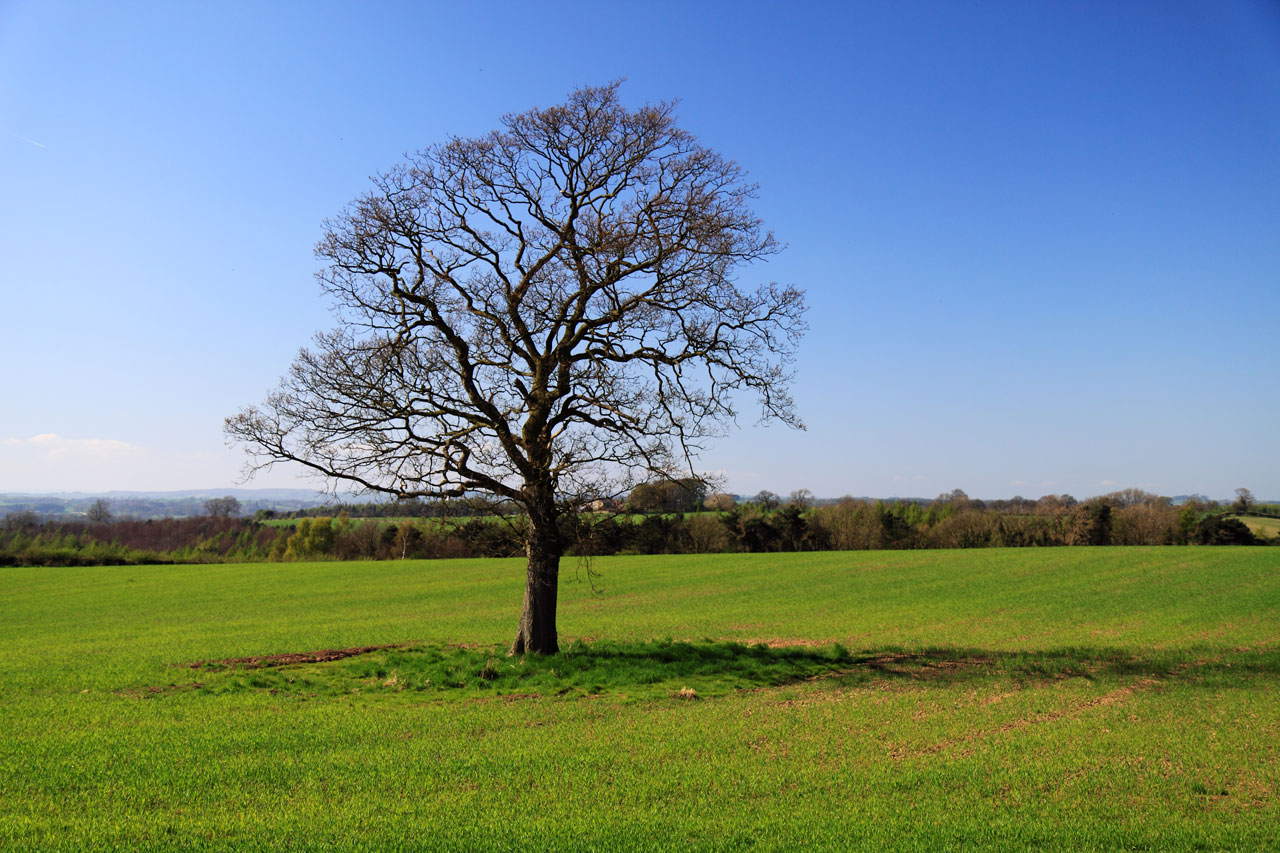
\includegraphics{lonely-tree}

That's all it take to insert a picture! The name of the picture without the
extension. \LaTeX will look for a picture with the name lonely-tree, in the
current directory or the path specified by \verb`\graphicspath`, in the formats
supported by pdflatex in our case.

For reference purposes those formats are: jpg, png, pdf and eps.

Not all tex installations can handle filenames with spaces. So it's better to
avoid them.

Notice that latex doesn't resize the picture to fit the document's size, and
that is not what you want most of the time, however the graphicx package has
some tools we'll cover in the next section to remedy that problem.


\section{Advanced}

\subsection{Scaling, resizing, rotating and trimming!}

\subsubsection{Scaling}
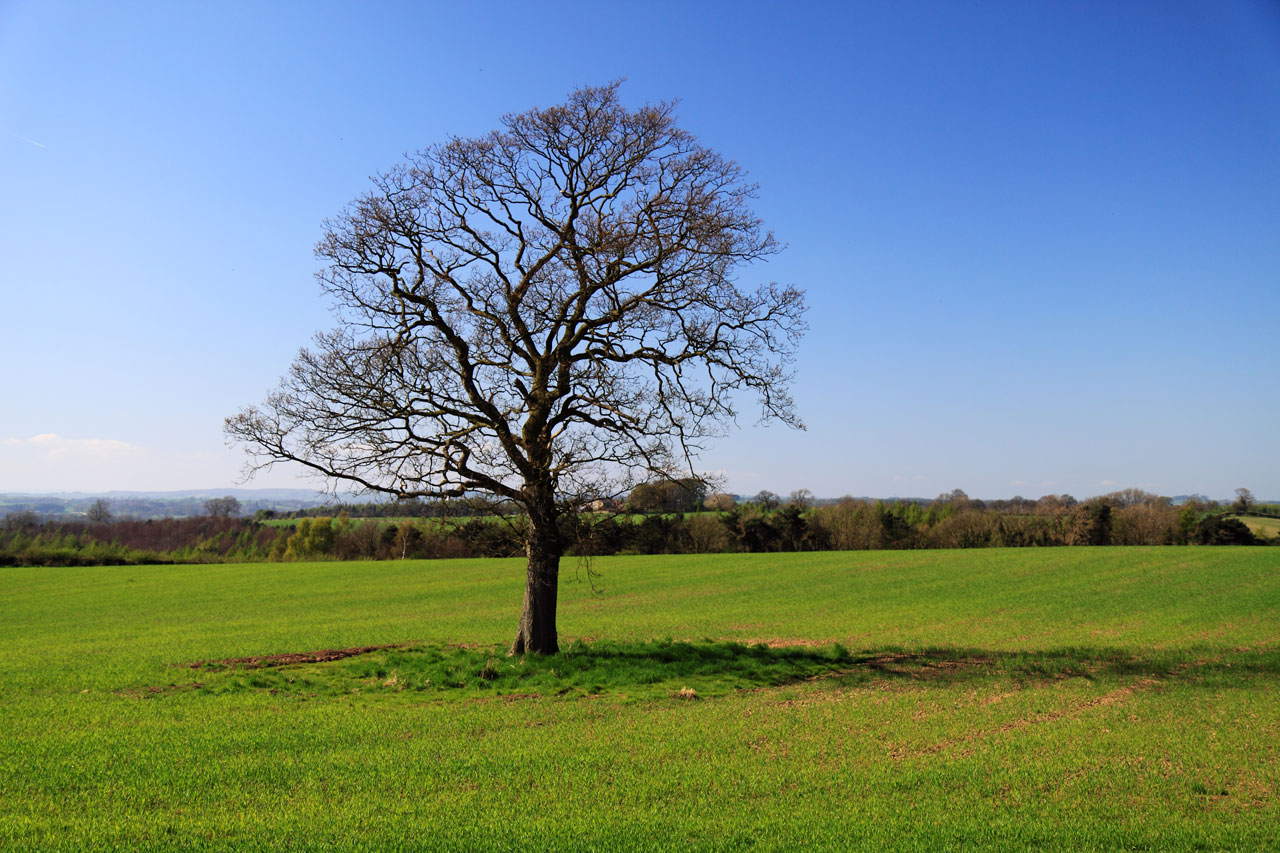
\includegraphics[scale=0.2]{lonely-tree}

You have the possibility to scale an image by a desired scale factor.
Here we multiply the dimensions by a factor of 0.2, or $\frac{1}{5}$,
effectively reducing the size by 5.


\subsubsection{Resizing}
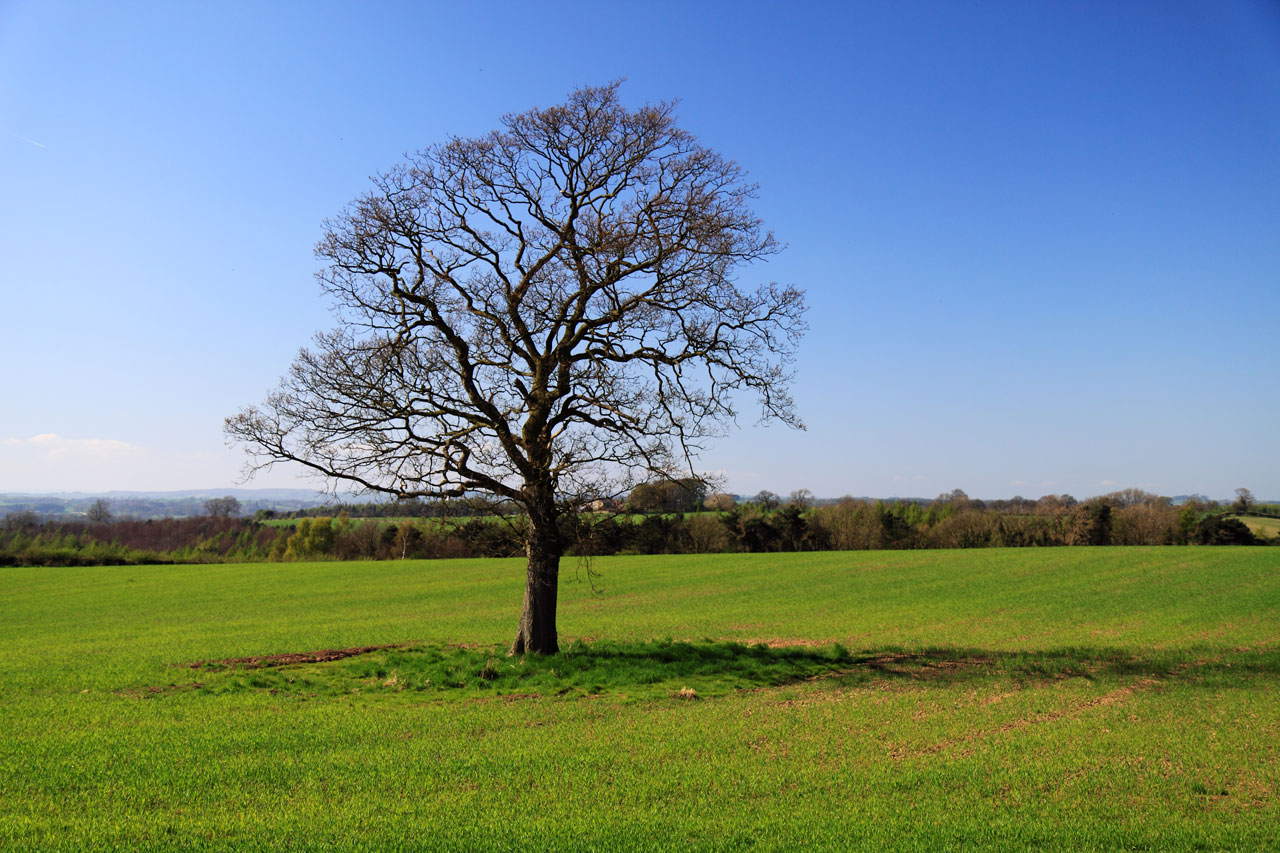
\includegraphics[width=5cm]{lonely-tree}
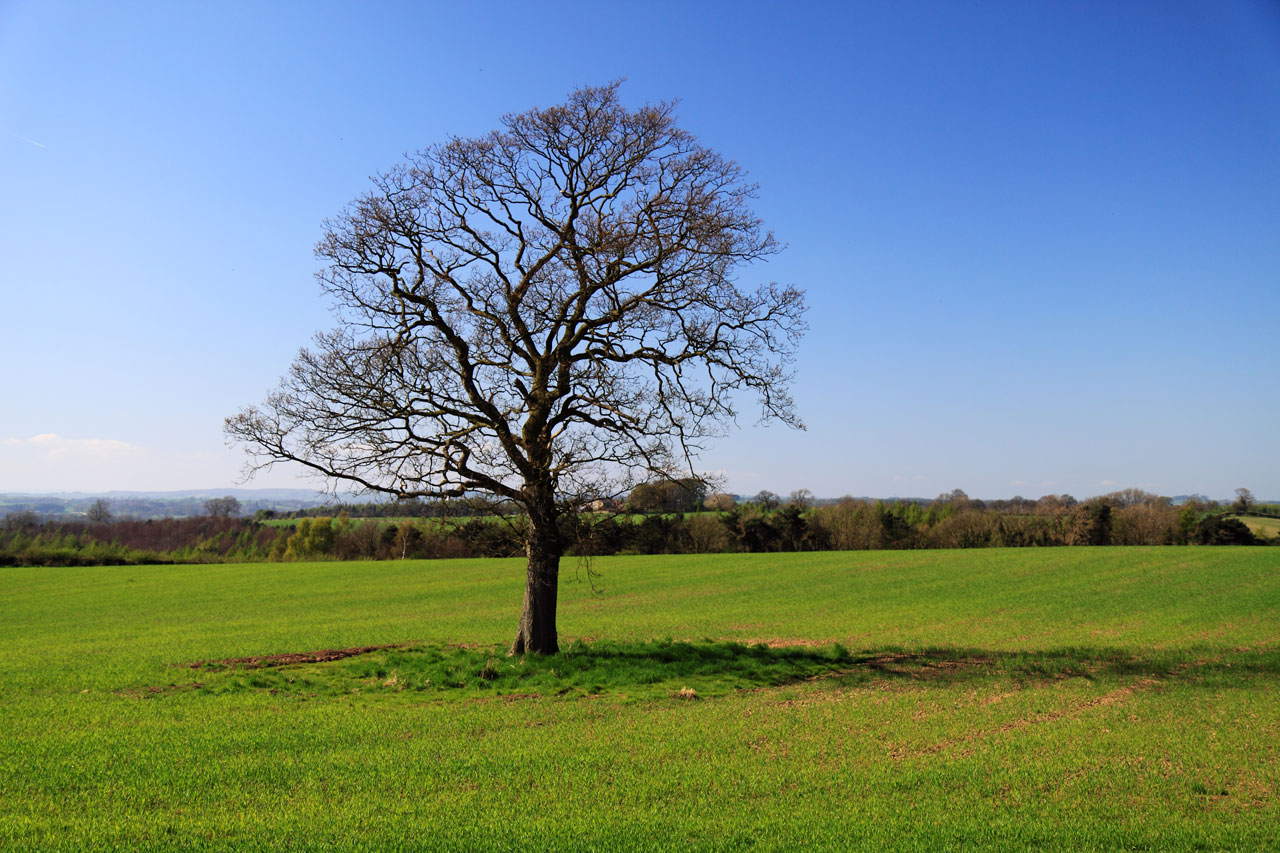
\includegraphics[height=5cm]{lonely-tree}

There might be a time you might want to scale a picture to a specific size, but
not necessarily know the factor by which you would have to multiply for scaling.
The solution here is using the \textit{width} and \textit{height} options of
the \verb`\includegrahics` command.

The above examples here set either the width or the height, and the picture
is scaled down to that size, respecting the aspect ratio.

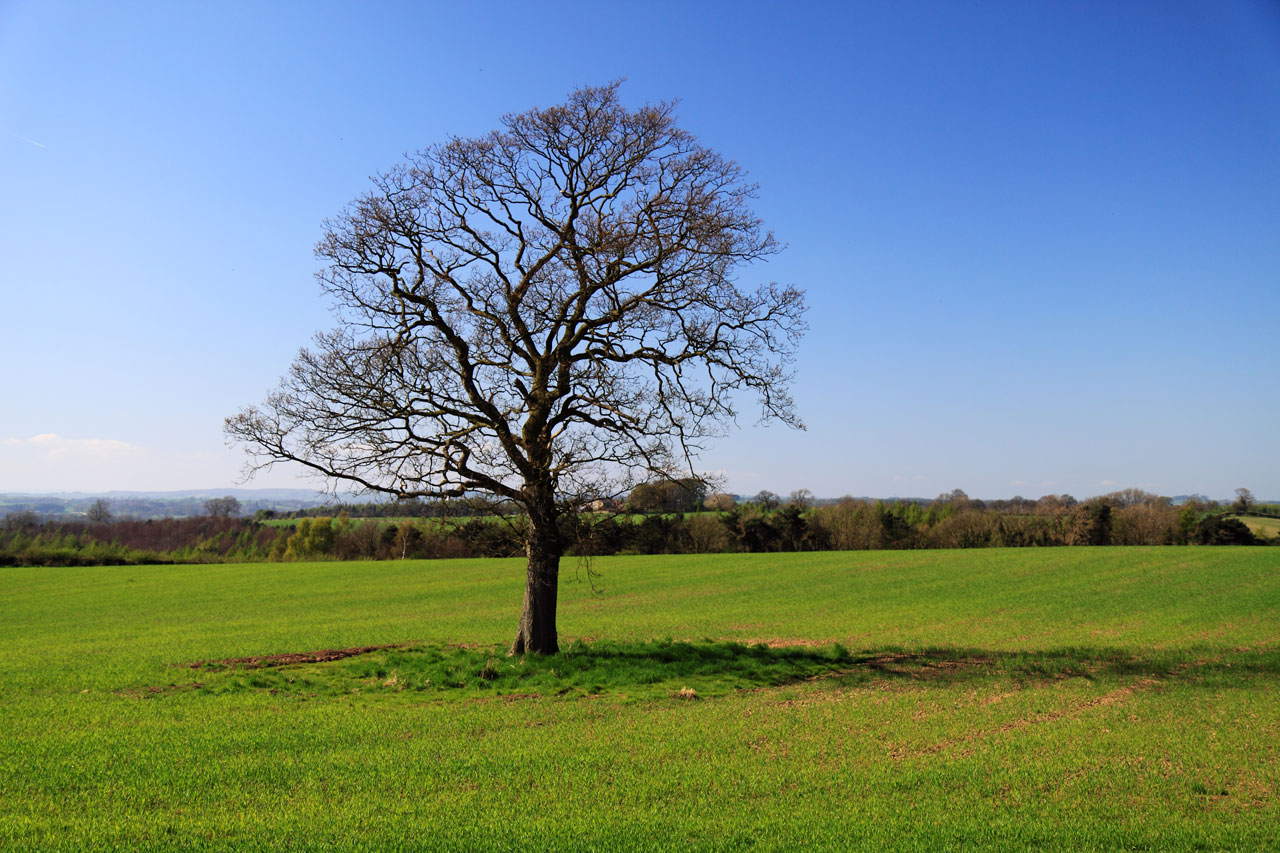
\includegraphics[width=5cm,height=5cm]{lonely-tree}
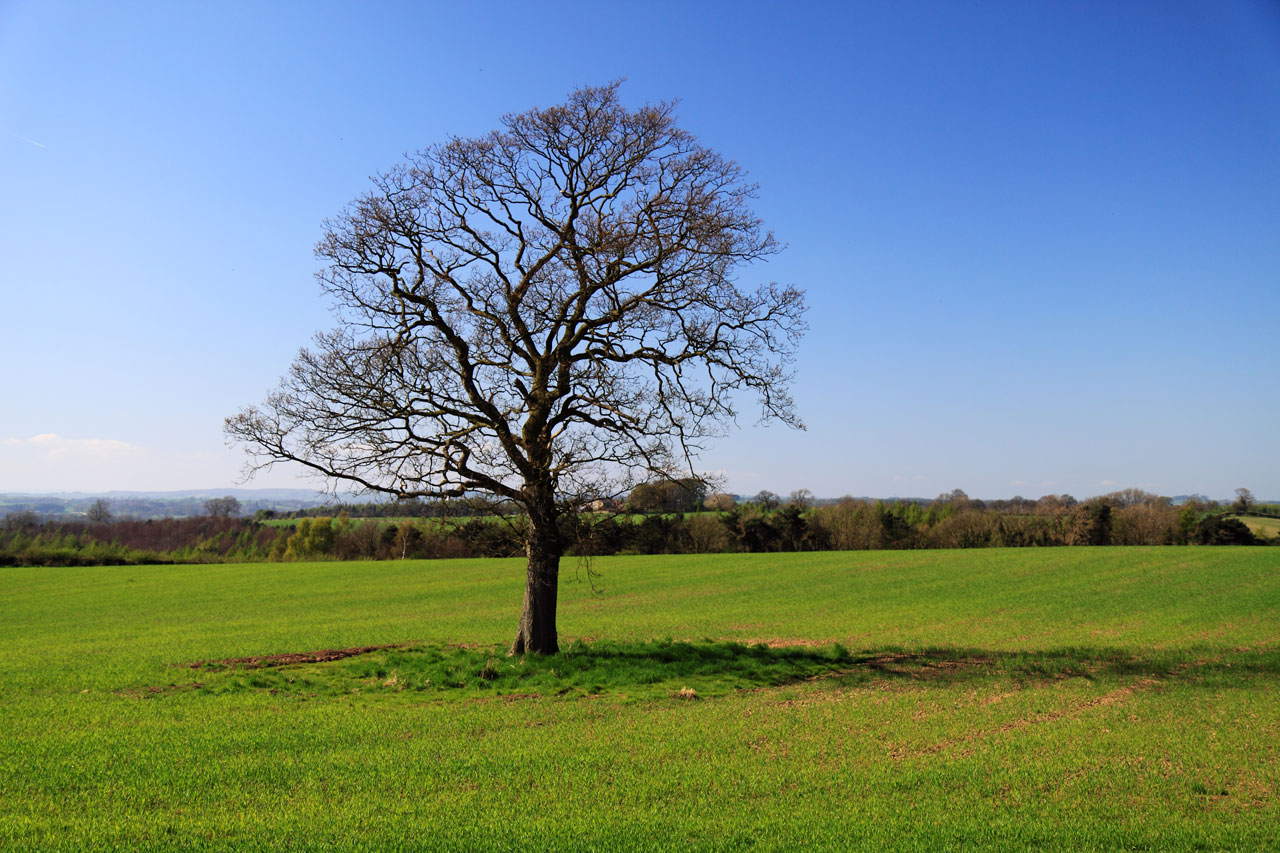
\includegraphics[width=5cm,height=5cm,keepaspectratio=true]{lonely-tree}

However, if both height and width are set, the image will be scaled according
to both height and width, and in case your original aspect ratio, is different
from the one specified through the \textit{width} and \textit{height} option,
the picture will distort.

If that behavior is undesirable, it's possible to use the
\textit{keepaspectratio=true} option in order to scale the picture according to
both width and height, and still keep the aspect ratio of the picture.


\subsubsection{Rotating}
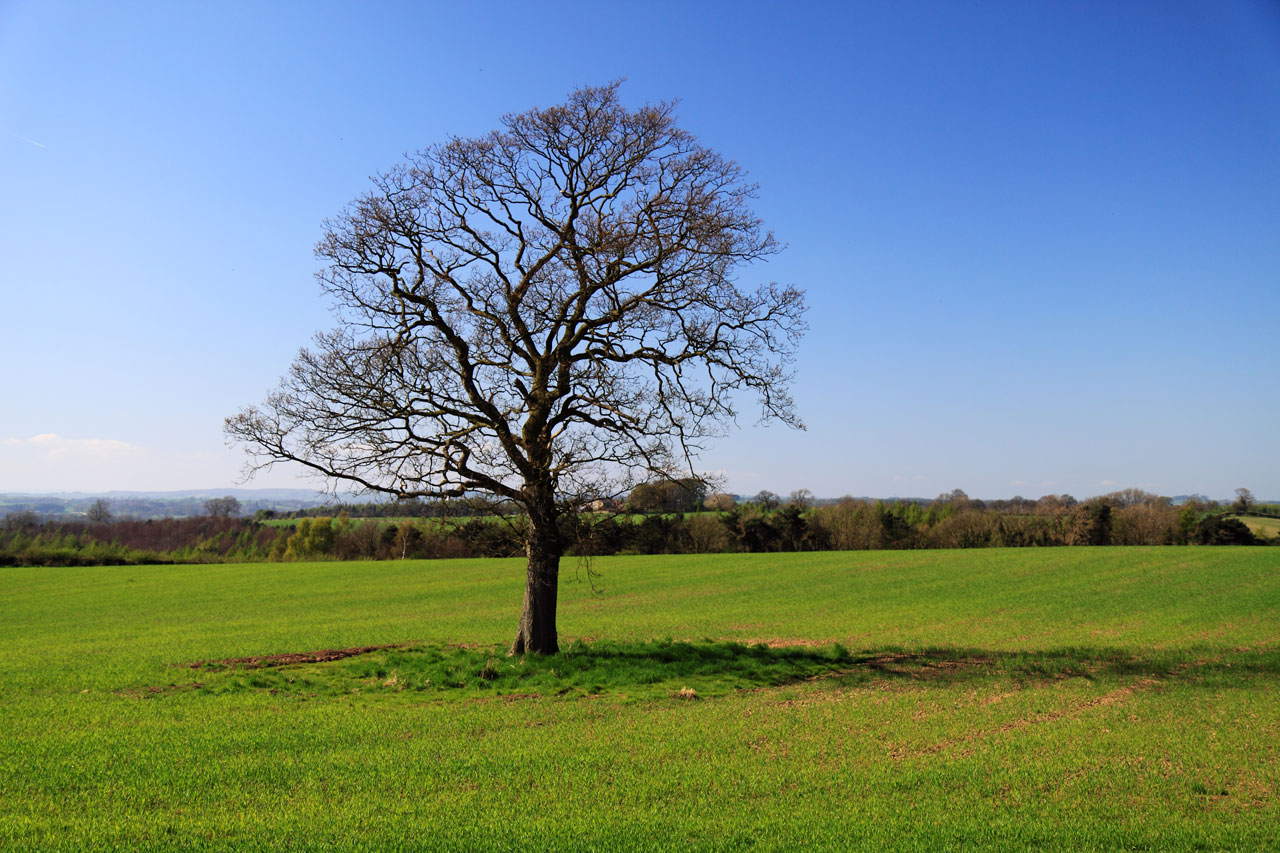
\includegraphics[width=5cm,angle=90]{lonely-tree}
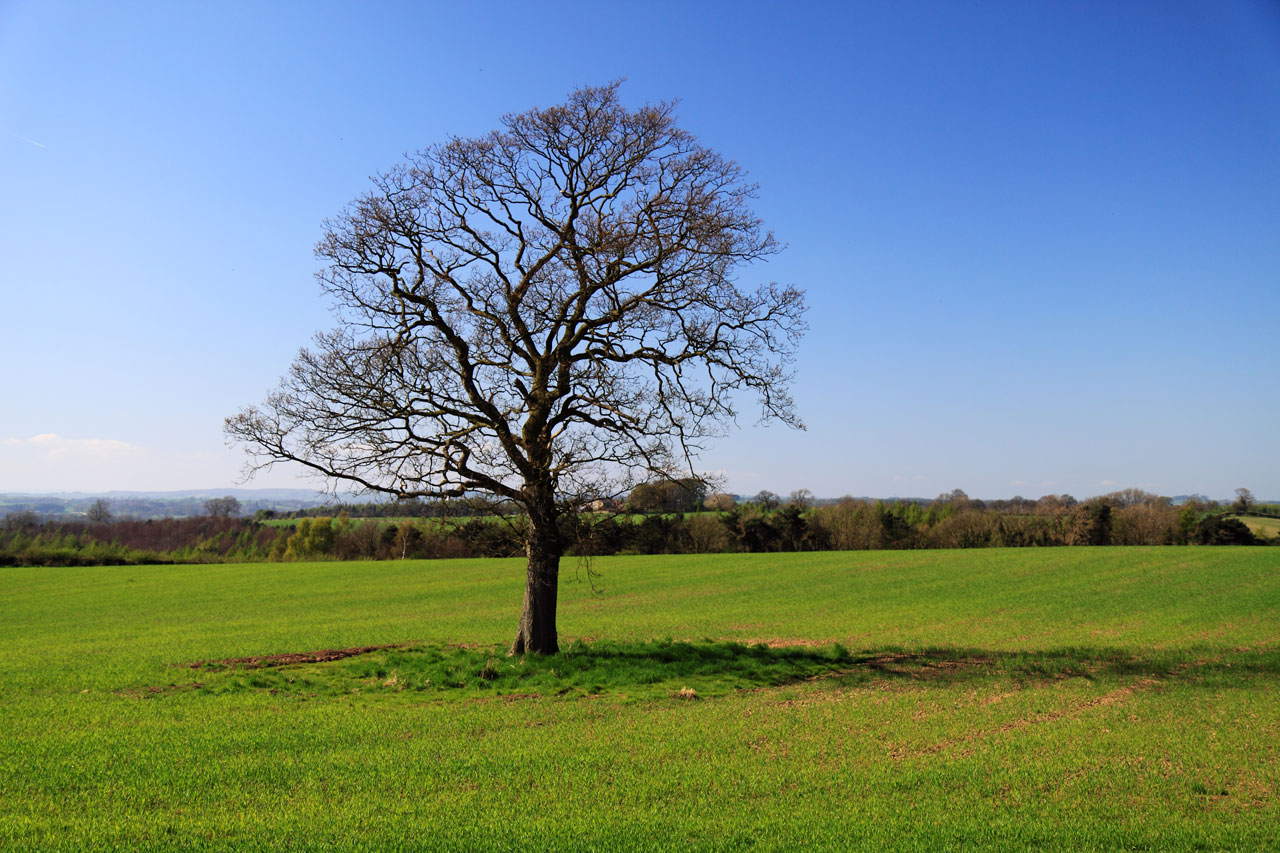
\includegraphics[width=5cm,angle=180]{lonely-tree}
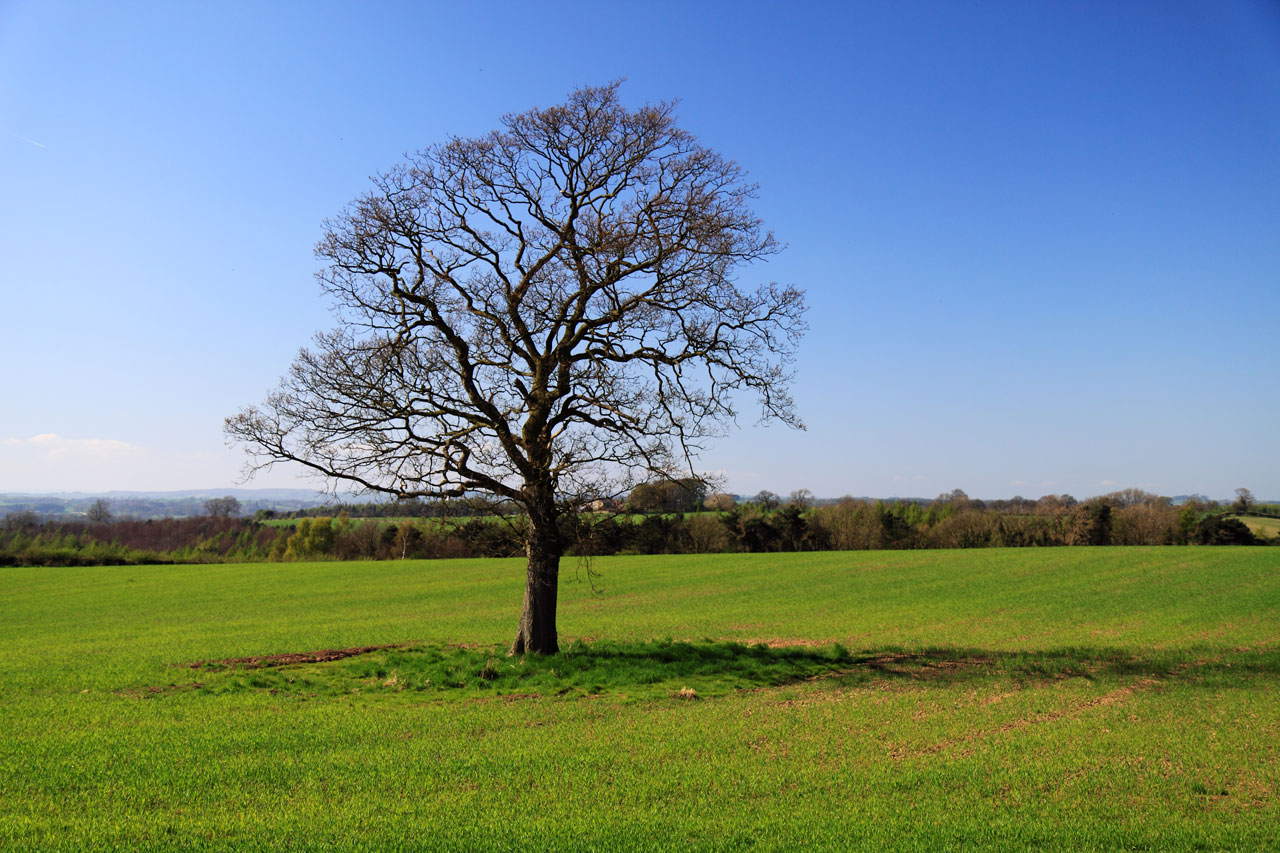
\includegraphics[width=5cm,angle=270]{lonely-tree}

The \textit{angle} option specifies by how much to rotate the image in degrees
counted \textbf{counter-clockwise}.

And as you can see, you can accumulate the scaling and rotating options.


\subsubsection{Trimming}
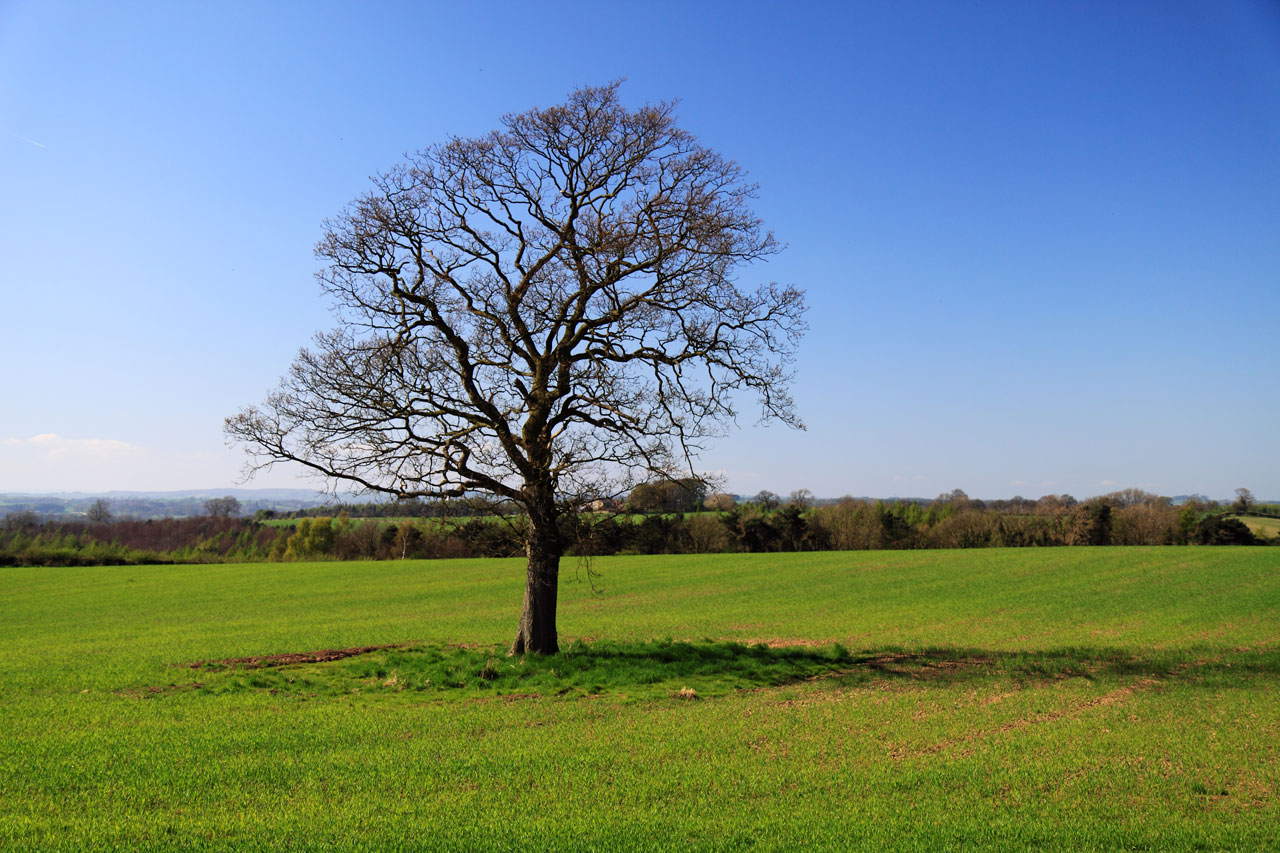
\includegraphics[height=5cm,trim=10mm 5mm 90mm 0mm,clip]{lonely-tree}

The \textit{trim=l b r t} option specifies by how much to trim on each side of
your picture, and the \textit{clip} option applies the trimming, effectively
cropping your picture.

This option will crop the included image by the lengths specified:
\textbf{l} from the \textit{left}, \textbf{b} from the \textit{bottom},
\textbf{r} from the \textit{right}, and \textbf{t} from the \textit{top}.

Note that the order for trimming is always counter-clockwise, starting on the
left.

You can accumulate scaling, rotating, and trimming, but notice that every time
while using those options, it applies to the original picture's state.


\subsection{Picture border}
\framebox{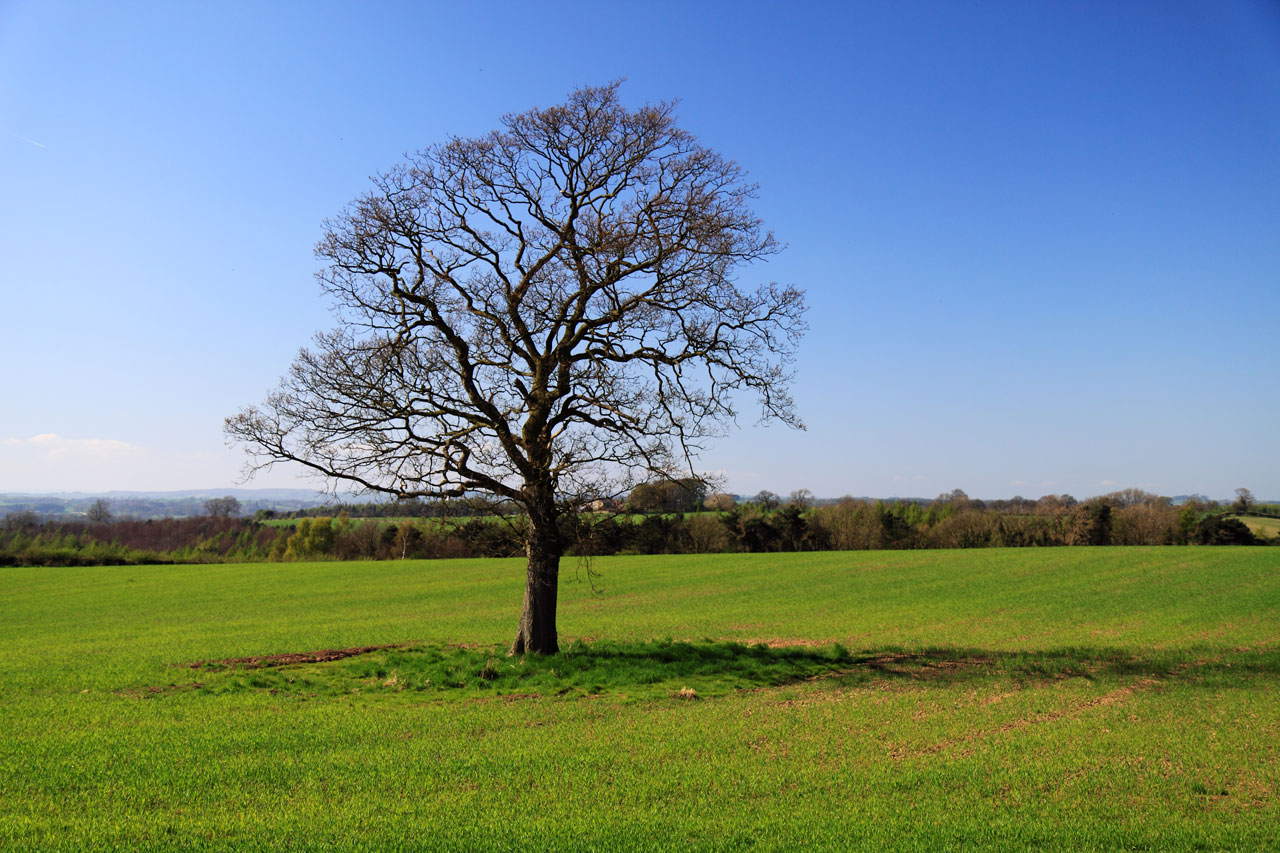
\includegraphics[width=5cm]{lonely-tree}}

\setlength\fboxsep{0pt}
\framebox{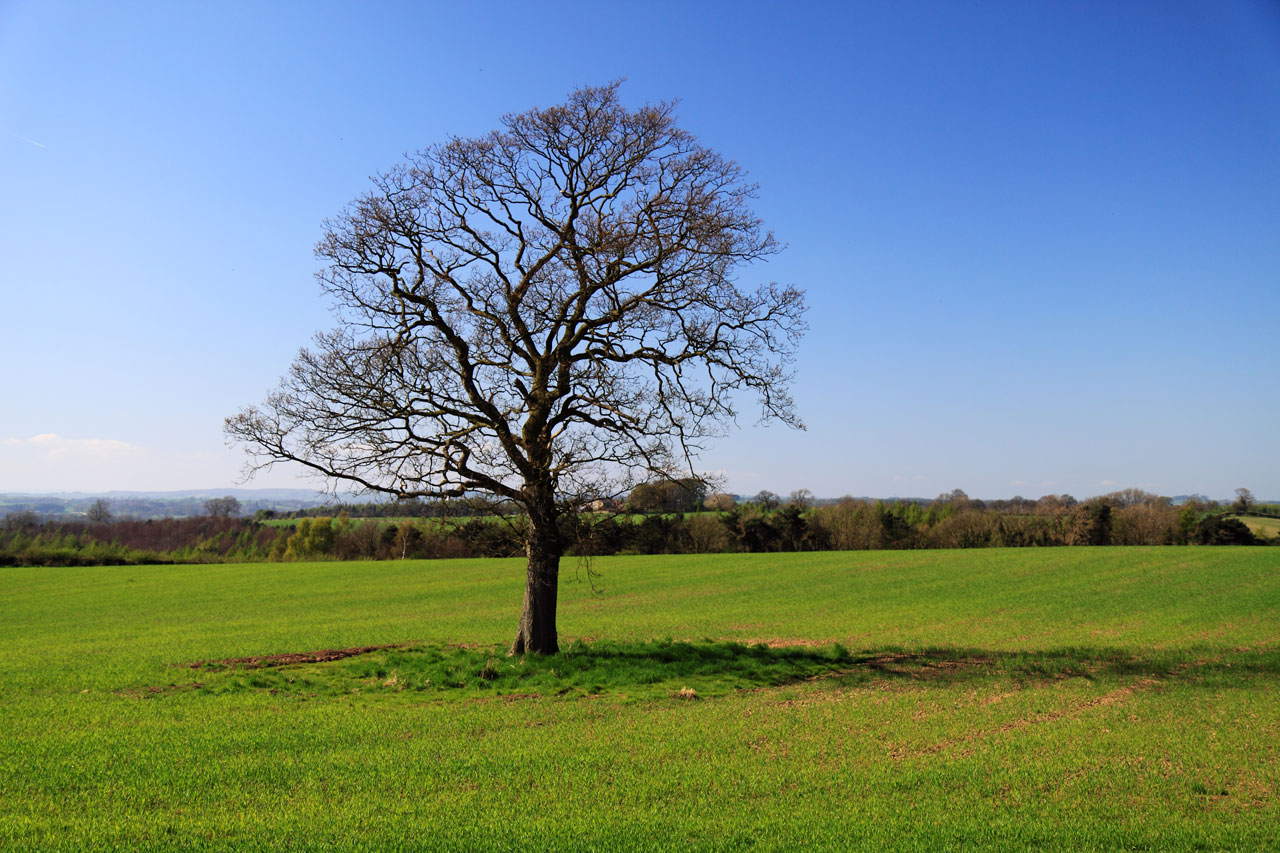
\includegraphics[width=5cm]{lonely-tree}}

\setlength\fboxsep{1pt}
\setlength\fboxrule{1pt}
\framebox{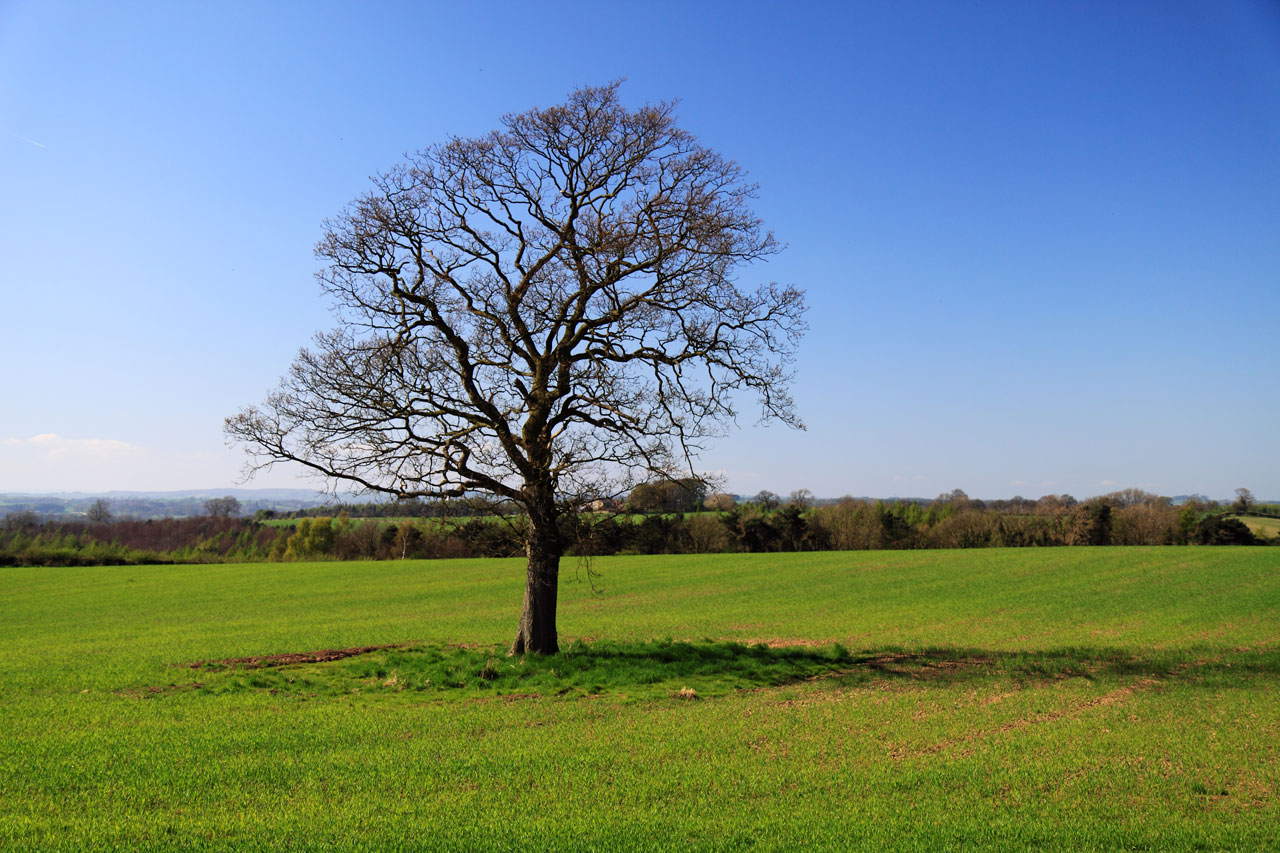
\includegraphics[width=5cm]{lonely-tree}}

The concept of boxes will be studied later, but right now, in order to have a
border around our picture, we'll be using a \textbf{framebox}, also shortened
as \textbf{fbox}.

To set a border around a picture simply use the \verb`\framebox` command,
passing your \verb`\includegraphics` command as an argument like in the example.

There are two aspects of a framebox we can adjust:
\begin{itemize}
    \item The margin between the content and the frame (or border), set in
    \verb`\fboxsep`, setting this to 0pts, will snap the border on the picture.
    \item The frame or border thickness, set in \verb`\fboxrule`.
\end{itemize}

Those aspects can be both set and modified using the \verb`\setlength` command
like in the examples above.


Using graphics \LaTeX can be fun but also tricky. For more information
concerning the graphics in \LaTeX, you should have a look in the
\href{official graphics guide}
{http://www.ctan.org/tex-archive/macros/latex/required/graphics/grfguide.pdf}.


\end{document}
